\documentclass[12pt]{article}
\usepackage[paper=letterpaper,margin=2cm]{geometry}

% images
\usepackage{graphicx}
\graphicspath{ {./images/} }

% multiple text columns
\usepackage{multicol}

\title{Neural encoding}
\author{Author: Daniel Gigliotti}
% \date{\today}
\date{}

\begin{document}
\maketitle

\section{Neural encoding and decoding}

In practice we won't be using the information about each individual action potential but rather the information coded into the frequency at which such action potentials are produced by the cell. We know almost exactly how a cell works but it's too complicated to account for that so we use a stochastic model.

\vspace{20px}

We will introduce two functions that can be associated with the output of a neuronal cell: the first, the `neural response function` is a precise description of the output; the second, the `firing rate` is more of an index summarizing the behaviour of the cell. We will introduce the central concept of `tuning curve` which is used to describe the behaviour of each individual neuron or of each family of neurons working simultaneously for the same purpose.

\vspace{20px}

Neural (En/De)coding: measuring and characterizing how an externl (for example light, sound, ...) or internal (for example an intent) input received by a neuron is translated into a sequence of action potentials (output) and vice versa.

\begin{center}
	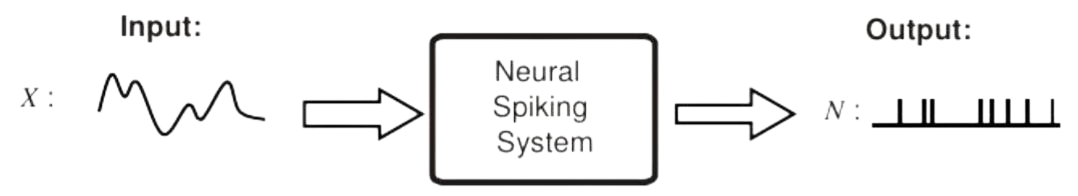
\includegraphics[scale=0.4]{images/neural_spiking_system.png}
\end{center}

\section{Neural encoding}

\begin{center}
    Encoding = finding a rule that leads from an input to an output.
\end{center}

\vspace{20px}

Encoding is done to understand the behaviour of a neuron in response to a particular input. Once we find that starting from a small set of sampled input data, we can do inference and predict its behaviour with data that the neuron hasn't seen yet; we can simulate the neuron with something that's artificial, thus simpler 

\begin{center}
	aim = describing how neurons react to different stimuli and trying to predict their response to a new one.
\end{center}

\begin{center}
	$neural\_response = f(stimulus)$
\end{center}

Once we find which property of the stimulus affects the most the neuronal response, we can understand the role of the neuron and its behaviour in a brain network.

\section{Neural decoding}

Neural decoding is the opposite procedure: from a neural response we need to go back to the inputs that induced it.

\begin{center}
	aim = recognize the stimulus (or its properties) that induced the spike train response
\end{center}

\begin{center}
$stimulus = f^{-1}(neural\_response)$
\end{center}

We can have several reasons to do that, like interface a device to our brain: in this case we must know how to interpret those signals and understand them.

\section{Concept}

We are going to summarize, to describe the behaviour of a single cell or an entire spiking system with a mathematical function, linking the input with the output.

\begin{center}
	Interesting bit of information: temporal distance between spikes
\end{center}

\section{Extended description $\rightarrow Neural\ response\ function$}

The extended description reports the exact sequence of action potentials that are produced by the cell. We can model a single spike as a Dirac $\delta$ function (impulse). To completely describe the output we can use this function:

\begin{center}
	$\rho (t) = \sum_{i=1}$ $\delta(t - t_i)$
	over $n$ spikes
\end{center}

This is a train of Dirac deltas, each of them centered on a specific time instance.

\section{Rate-coding hypothesis}

The rate-coding hypothesis suggests that spike frequency (or rate) is the fundamental mechanism of coding information.

According to this hypothesis, the information relies in the temporal distance between different action potentials $\rightarrow$ if sufficiently near, in the post-synaptic neuron they will produce a temporal summation and a stronger stimulus.

\section{Synthetic description $\rightarrow Firing\ rate$}

Instead of the previous formula, still too complex, we will use the \emph{firing rate}, an index that measures the effect that the neuronal output will have on the following cells; the higher the firing rate, the higher the temporal summation and the post-synaptic potentials will be.

The spike-count firing rate is the time average of the neural response function over the duration of the trial.

\begin{center}
	$r = \frac{n}{T} = \int_{0}^{T} \rho(\tau) d\tau$
\end{center}

We can use the spike-count firing rate when the stimulus is stationary, so we can average multiple ($n$) trials, each with duration $T$, in order to have a more consistent measurement.

\begin{center}
	$\left \langle r \right \rangle = \frac{\left \langle n \right \rangle}{T} = \frac{1}{T}\int_{0}^{T}r(t) dt$
\end{center}

\section{Tuning curves}

\begin{center}
	$\left \langle r \right \rangle = f(s)$
	where $s$ is a single property assumed stationary along each trial (repeated stimulation)
\end{center}

$f(s)$ will be empirically obtained:

\begin{enumerate}
	\item provide stimulus and measure the output (in vivo - we don't need too much precision -, non invasively);
	\item analyze the output of the cell (e.g. average);
	\item plot the availabe data;
	\item find the function that better approximates it;
\end{enumerate}

\section{Stochastic models}

The relation between a given stimulus property $s$ and the generation of a single action potential is too complex to be modeled. 

We need a statistical model that allows us to estimate the probability of an arbitrary spike sequence occurring, based on our knowledge of the responses actually recorded (firing rate $r$).

If the probability of generating an action potential is independent of the presence or timing of other spikes, the firing rate $r$ is all we need to compute the probabilities for all possible action potential sequences. An extremely useful approximation of stochastic neuronal firing is provided by the Poisson process:

\begin{itemize}
	\item homogeneous, when the firing rate $r$ is constant over time
	\item inhomogeneous, for a time-dependent firing rate $r(t)$
\end{itemize}

We will focus on the homogeneous $Poisson\ process$.

\section{Homogeneous Poisson process}

\begin{center}
	$P_T[n] = \frac{(rT)^n}{n!}e^{-rT}$
\end{center}

$P_T[n]$ is the probability of $n$ spikes occurring during a trial of length $T$.
$r$ is the firing rate (usually the average over trials $\left \langle r \right \rangle$)
$rT$ is the average (across trials) number of spikes in $T$

When $T$ increases, higher values of $n$ are more likely; the same applies when $r$ increases.

\section{The inter-spike interval distribution}

We divide the trial $T$ in very small time intervals $\Delta t (\rightarrow 0)$ so that no more than a single spike can occur in each interval. An action potential is called $event$.

Given a spike at $t_i$, we want to know the probability of the following spike to be produced (event) in the interval $\tau$:

\begin{center}
	$t_i + \tau \leq t_{i+1} \leq t_i + \tau + \Delta t$
\end{center}


This is equal to:

\begin{center}
	probability of no spike for a time $\tau$ * probability of a spike in $\Delta t$
\end{center}

\begin{itemize}

	\item Probability of no spike in $\tau$:
		\begin{center}
			$n = 0$
		\end{center}
		\begin{center}
			$T = \tau$
		\end{center}

		In the Poisson distribution:

		\begin{center}
			$P_T[n] = \frac{(rT)^n}{n!}e^{-rT} \rightarrow \frac{(r \tau)^0}{0!}e^{-r \tau} \rightarrow e^{-rT}$ 
		\end{center}

	\item Probability of a spike in $\Delta t$:
		\begin{center}
			$\Delta t = r \Delta t$
		\end{center}
\end{itemize}

Finally:

\begin{center}
	inter-spike interval distribution
	$t_i + \tau \leq t_{i+1} \leq t_i + \tau + \Delta t = r \Delta t e^{-r \tau}$
\end{center}

The most likely inter-spike intervals are short ones; long intervals have a probability that falls exponentially as a function of their duration.

\section{The Poisson spike generator}

Procedure:

\begin{enumerate}
    \item experimental estimation of the firing rate $r_{est}$ (tuning curve);
    \item build a spike generator based on a Poisson distribution with $r = r_{est}$;
\end{enumerate}

\vspace{20px}

\noindent
A Poisson spike generator is a simple algorithm that a computer can run:

\renewcommand{\labelenumii}{\theenumii}
\renewcommand{\theenumii}{\theenumi.\arabic{enumii}.}

\begin{enumerate}
    \item the program progresses through time in small steps of size $\Delta t$;
    \item for each time step $\Delta t$:
    \begin{enumerate}
        \item it generates a random number $x_{rand}$ chosen uniformly in the range $[0, 1]$ (threshold, independent from $r$);
        \item uf $r_{est} \Delta t > x_{rand}$ a spike is fired in this time step, otherwise is not;
    \end{enumerate}
\end{enumerate}

The threshold $x_{rand}$ is fixed for each time step.

\vspace{20px}

When ISI (inter-spike interval) is very low, data don't align with the exponential rule. The problem is that we don't account for the refractory period: two consecutive spikes are not completely independent in real life soon, they get independent after a while. In the actual neuron, the minimum inter-spike distance is constrained.

\vspace{20px}

Note: 
\begin{enumerate}
	\item absolute refractory period (repolarization) is due to the $Na^+$ voltage-gated channels inactivation. No new action potential can be produced under any circumstance;
	\item relative refractory period (hyperpolarization) is due to the $K^+$ voltage-gated channels; a new action potential can be produced, but it requires a stronger depolarization $\rightarrow$ it's less likely to occur.
\end{enumerate}

\end{document}
